En Álgebra I el objeto principal de estudio fueron los anillos conmutativos, conjuntos en los que teníamos definidas dos operaciones, una usualmente denotada con notación aditiva y otra con notación multiplicativa.

Posteriormente, el estudio se centró en los dominios de integridad (DI), anillos conmutativos donde teníamos más propiedades con las que manejar nuestros elementos (como la tan característica propiedad cancelativa). Después, el objeto de estudio fueron los dominios euclídeos (DE), donde ya podíamos realizar un estudio sobre la divisibilidad de los elementos del conjunto.

Finalmente, nos centramos en los dominios de factorización única (DFU), donde realizamos una breve introducción a la irreducibilidad de los polinomios.\\

En esta asignatura el principal objeto de estudio serán los grupos, conjuntos en los que hay definida una sola operación que entendemos por ``buena\footnote{La operación cumplirá ciertas propiedades deseables.}''. Por tanto, los grupos serán estructuras menos restrictivas que los anillos conmutativos, aunque su estudio no será menos interesante.

\chapter{Grupos: definición, generalidades y ejemplos}
Comenzamos realizando la primera definición necesaria para entender el concepto de grupo, que es entender qué es una operación dentro de un conjunto.

\begin{definicion}[Operación binaria]
    Sea $G$ un conjunto, una operación binaria en $G$ es una aplicación
    \Func{\ast}{G\times G}{G}{(a,b)}{a\ast b}
\end{definicion}

\begin{ejemplo}
    Ejemplos de operaciones binarias sobre conjuntos que ya conocemos son:
    \begin{enumerate}
        \item La suma y el producto de números en $\mathbb{N}$, $\mathbb{Z}$, $\mathbb{Q}$, $\mathbb{R}, \mathbb{C}$.
        \item Dado un conjunto $X$, los operadores $\cap$ y $\cup$ son operaciones binarias sobre el conjunto $\mathcal{P}(X)$.
    \end{enumerate}
\end{ejemplo}

% // TODO: Descomentar lo de monoide cuando se sepa seguro
% Antes de dar la definición de grupo, daremos la de monoide, que es menos restrictiva que la de grupo.

% \begin{definicion}[Monoide]
%     Un monoide es una tripleta $(G,\ast,e)$ donde $G$ es un conjunto no vacío, $\ast$ es una operación binaria en $G$ y $e$ es un elemento destacado de $G$ de forma que se verifica:
%     \begin{enumerate}
%         \item[$i)$] La propiedad asociativa de $\ast$:
%             \begin{equation*}
%                 (x\ast y) \ast z = x \ast (y\ast z) \qquad \forall x,y,z\in G
%             \end{equation*}
%             % // TODO: No es seguro, pero probablemente es necesario exigir x * e = x
%         \item[$ii)$] La existencia de un elemento neutro (el elemento destacado de $G$):
%             \begin{equation*}
%                 \exists e\in G \mid e\ast x = x \qquad \forall x\in G
%             \end{equation*}
%     \end{enumerate}
% \end{definicion}

% % // TODO: Revisar esto a partir de la definición
% \begin{observacion}
%     En un monoide, el elemento neutro es único.
%     \begin{proof}
%         Sea $(G,\ast,e)$ un monoide y sea $f\in G$ tal que $f\ast x = x$ $\forall x\in G$:
%     \end{proof}
% \end{observacion}

% \begin{ejemplo}
%     Ejemplos de monoides ya conocidos son:
%     \begin{enumerate}
%         \item $(\mathbb{N}, +, 0)$, $(\mathbb{N}, \cdot, 1)$
%         \item Dado un conjunto $X$: $(\mathcal{P}(X), \cap, X)$, $(\mathcal{P}(X), \cup, \emptyset )$
%     \end{enumerate}
% \end{ejemplo}

\begin{definicion}[Grupo]
    Un grupo es una tripleta $(G,\ast,e)$ donde $G$ es un conjunto no vacío, $\ast$ es una operación binaria en $G$ y $e$ es un elemento destacado de $G$ de forma que se verifica:
    \begin{enumerate}
        \item[$i)$] La propiedad asociativa de $\ast$:
            \begin{equation*}
                (x\ast y) \ast z = x \ast (y\ast z) \qquad \forall x,y,z\in G
            \end{equation*}
        \item[$ii)$] La existencia de un elemento neutro (el elemento destacado de $G$):
            \begin{equation*}
                \exists e\in G \mid e\ast x = x \qquad \forall x\in G
            \end{equation*}
        \item[$iii)$] La existencia de un elemento simétrico para cada elemento de $G$:
            \begin{equation*}
                \forall x\in G \quad \exists x'\in G\mid x'\ast x = e
            \end{equation*}
    \end{enumerate}
    Si además se cumple:
    \begin{enumerate}
        \item[$iv)$] La propiedad conmutativa de $\ast$: 
            \begin{equation*}
                x\ast y = y \ast x \qquad \forall x,y\in G
            \end{equation*}
    \end{enumerate}
    Entonces, diremos que $(G,\ast,e)$ es un grupo conmutativo o abeliano.
\end{definicion}

\begin{notacion}
    Para una mayor comodidad a la hora de manejar grupos, introducimos las siguientes notaciones:
    \begin{enumerate}
        \item Cuando dado un conjunto no vacío $G$ sepamos por el contexto a qué grupo $(G,\ast,e)$ nos estamos refiriendo, indicaremos simplemente $G$ (o en algunos casos $(G,\ast)$, para hacer énfasis en la operación binaria) para referirnos al grupo $(G,\ast,e)$.
        \item En algunos casos, usaremos (por comodidad) la notación multiplicativa de los grupos. De esta forma, dado un grupo $(G,\cdot,1)$, en ciertos casos notaremos la operación binaria $\cdot$ simplemente por yuxtaposición:
            \begin{equation*}
                x \cdot y = xy \qquad \forall x,y\in G
            \end{equation*}
            Además, nos referiremos al elemento neutro como ``uno'' y al simétrico de cada elemento como ``inverso'', sustituyendo la notación de $x'$ por la de $x^{-1}$.
        \item Otra notación que también usaremos (aunque de forma menos frecuente que la multiplicativa) será la aditiva. Dado un grupo $(G,+,0)$, nos referiremos al elemento neutro como ``cero'' y al simétrico de cada elemento como ``opuesto'', sustituyendo la notación de $x'$ por la de $-x$.
    \end{enumerate}
\end{notacion}

\begin{ejemplo} Ejemplos de grupos que se usarán con frecuencia en la asignatura son:
     \begin{enumerate}
         \item $\mathbb{Z},\mathbb{Q},\mathbb{R},\mathbb{C}$ con su respectiva suma son grupos abelianos.
         \item $\mathbb{Q}^\ast,\mathbb{R}^\ast,\mathbb{C}^\ast$ con su respectivo producto son grupos abelianos.

             Notemos la importancia de eliminar el $0$ de cada conjunto para que todo elemento tenga inverso, así como que $\mathbb{Z}^\ast$ no es un grupo, ya que el inverso de cada elemento (para el producto al que estamos acostumbrados) no está dentro de $\mathbb{Z}^\ast$.
         \item $\{1,-1,i,-i\}\subseteq \mathbb{C}$ con el producto heredado\footnote{Será común hablar de ``operación heredada'' cuando consideramos un subconjunto de un conjunto en el que ya hay definida una operación interna, haciendo referencia a la restricción en dominio y recorrido de dicha operación interna al subconjunto considerado.} de $\mathbb{C}$ también es un grupo abeliano.
         \item $(\mathcal{M}_2(\mathbb{R}),+)$ es un grupo abeliano.
         \item El grupo lineal de orden 2 con coeficientes en $\mathbb{R}$:
             \begin{equation*}
                 GL_2(\mathbb{R}) = \{M\in \mathcal{M}_2(\mathbb{R}) : det(M)\neq 0\}
             \end{equation*}
             con el producto heredado de $\mathcal{M}_2(\mathbb{R})$ es un grupo abeliano.
         \item $\mathbb{Z}_n$ con su suma es un grupo abeliano, $\forall n\in \mathbb{N}$.
         \item $U(\mathbb{Z}_n)=\{[a]\in \mathbb{Z}_n \mid mcd(a,n)=1\}$ con el producto es un grupo abeliano, $\forall n\in \mathbb{N}$.
         \item Dado $n\geq 1$, consideramos:
             \begin{align*}
                 \mu_n &= \{\text{raíces complejas de\ } x^n-1\} = \left\{\xi_n = \cos\frac{2k\pi}{n} + i\sen\frac{2k\pi}{n}\right\} \\
                       &= \left\{1,\xi,\xi^2, \ldots, \xi^{n-1} : \xi = \cos\frac{2\pi}{n} + i\sen\frac{2\pi}{n}\right\}
             \end{align*}
             Es un grupo abeliano con el producto heredado de $\mathbb{C}$.
         \item Dado un cuerpo $\mathbb{K}$, el grupo lineal especial de orden 2 sobre dicho cuerpo:
             \begin{equation*}
                 SL_2(\mathbb{K}) = \{M\in \mathcal{M}_2(\mathbb{K}) : det(M) = 1\}
             \end{equation*}
             Con el producto heredado de $\mathcal{M}_2(\mathbb{K})$ es un grupo que no es conmutativo.
         \item Sean $(G,\square,e),(H,\triangle,f)$ dos grupos, si consideramos sobre $G\times H$ la operación binaria $\ast:(G\times H)\times(G\times H)\rightarrow G\times H$  dada por:
             \begin{equation*}
                 (x,u) \ast (y,v) = (x\square y, u\triangle v) \qquad \forall (x,u),(y,v)\in G\times H
             \end{equation*}
             Entonces, $G\times H$ es un grupo, al que llamaremos \underline{grupo directo} de $G$ y $H$.
         \item Si $X$ es un conjunto no vacío y consideramos
             \begin{equation*}
                 S(X) = \{f:X\rightarrow X \mid f \text{\ biyectiva}\} = Perm(X)
             \end{equation*}
             es un grupo no abeliano con la operación de composición de funciones $\circ$.

             En el caso en el que $X$ sea finito y tenga $n$ elementos: $X = \{x_1, x_2, \ldots, x_n\}$, notaremos:
             \begin{equation*}
                 S_n = S(X)
             \end{equation*}
         \item Sea $(G,\ast,e)$ un grupo y $X$ un conjunto, consideramos el conjunto:
             \begin{equation*}
                 Apl(X,G) = G^X = \{f:X\rightarrow G \mid f \text{\ aplicación}\}
             \end{equation*}
             junto con la operación binaria $\ast:G^X\times G^X \rightarrow G^X$ dada por:
             \begin{equation*}
                 (f\ast g)(x) = f(x)\ast g(x) \qquad \forall x\in X, \quad \forall f,g\in G^X
             \end{equation*}
             Entonces, $(G^X, \ast, g)$ es un grupo, con elemento neutro:
             \begin{equation*}
                 g(x) = e \qquad \forall x\in X
             \end{equation*}
             de esta forma, dada $f\in G^X$, la aplicación simétrica de $f$ será:
             \begin{equation*}
                 f'(x) = {(f(x))}' \qquad \forall x\in X
             \end{equation*}

             Casos a destacar son:
             \begin{enumerate}
                 \item Si $X=\emptyset $, entonces $G^X = \{\emptyset \}$.
                 \item Si $X = \{1,2\}$, entonces $G^X$ se identifica con $G\times G$.
             \end{enumerate}
         \item El grupo más pequeño que se puede considerar es el único grupo válido sobre un conjunto unitario $X=\{e\}$. Es decir, el grupo $(X,\ast,e)$ con $X = \{e\}$ y $\ast:X\times X\rightarrow X$ dada por:
             \begin{equation*}
                 e\ast e = e \qquad e\in X
             \end{equation*}
             A este grupo (independientemente de cual sea el conjunto $X$, ya que todos tendrán la misma\footnote{Concepto que luego formalizaremos.} estructura) lo llamaremos \underline{grupo trivial}.
     \end{enumerate}
\end{ejemplo}

\subsubsection{Propiedades}
Aunque estas propiedades parezcan ya conocidas y familiares (por ejemplo para el caso $(\mathbb{Z},+,0)$), es una buena observación darnos cuenta de que son válidas para \textbf{cualquier grupo} que consideremos, por raros y difíciles que sean sus elementos y operación interna.

\begin{prop}
    Sea $(G,\ast,e)$ un grupo, destacamos sus primeras propiedades:
    \begin{enumerate}
        \item[$i)$] $x\ast x' = e$ $\forall x\in G$.
        \item[$ii)$] $x\ast e = x$ $\forall x\in G$.
        \item[$iii)$] El elemento neutro de $\ast$ es único. Simbólicamente:
            \begin{equation*}
                \exists_1 e\in G \mid e\ast x = x \qquad \forall x\in G
            \end{equation*}
        \item[$iv)$] Fijado $x\in G$, el simétrico de $x$ es único. Simbólicamente:
            \begin{equation*}
                \forall x\in G \quad \exists_1 x' \in G \mid x' \ast x = e
            \end{equation*}
    \end{enumerate}
    \begin{proof}
        Demostramos cada una a partir de la anterior:
        \begin{enumerate}
            \item[$i)$] En primer lugar, observemos que:
                \begin{equation}\label{eq:primera_ec}
                    x'\ast (x\ast x') = (x'\ast x) \ast x' = e \ast x' = x'
                \end{equation}
                Ahora:
                \begin{equation*}
                    x\ast x' = e\ast (x \ast x') = \left({(x')}'\ast x'\right) \ast (x\ast x') = {(x')}' \ast (x'\ast (x\ast x')) \AstIg {(x')}' \ast x' = e
                \end{equation*}
                Donde en $(\ast)$ hemos usado~(\ref{eq:primera_ec}).
            \item[$ii)$] Usando $i)$ en $(\ast)$:
                \begin{equation*}
                    x\ast e = x\ast (x' \ast x) = (x \ast x') \ast x \AstIg e \ast x = x
                \end{equation*}
            \item[$iii$)] Sea $f\in G$ de forma que $f\ast x = x$ $\forall x\in G$, entonces:
                \begin{equation*}
                    f = f \ast e \AstIg e
                \end{equation*}
                Donde en $(\ast)$ hemos usado $ii)$.
            \item[$iv)$] Dado $x\in G$, sea $x'' \in G$ de forma que $x'' \ast x = x$, entonces:
                \begin{equation*}
                    x '' = x'' \ast e \AstIg x '' \ast (x \ast x') = (x '' \ast x) \ast x' = e \ast x' = x'
                \end{equation*}
                Donde en $(\ast)$ hemos usado $i)$.
        \end{enumerate}
    \end{proof}
\end{prop}

\begin{notacion}
    A partir de ahora, dado un grupo $(G,\ast,e)$, comenzaremos a usar (por comodidad) la notacion multiplicativa de los grupos:
    \begin{equation*}
        xy = x\ast y \qquad \forall x,y\in G
    \end{equation*}
    Y denotando a $x'$ (el elemento simétrico de $x$) por $x^{-1}$.
\end{notacion}

\begin{prop}
    En un grupo $G$ se verifica la propiedad cancelativa (tanto a la izquierda como a la derecha):
    \begin{equation*}
        \forall x,y,z\in G:\ \left\{\begin{array}{l}
            xy = xz \Longrightarrow y = z \\
            xy = zy \Longrightarrow x = z
        \end{array}\right.
    \end{equation*}
    \begin{proof}
        Para la primera, supongamos que $xy=xz$:
        \begin{equation*}
            y = ey = (x^{-1}x)y = x^{-1}(xy) = x^{-1}(xz) = (x^{-1}x)z = ez = z
        \end{equation*}
        Ahora, para la segunda, supongamos que $xy = zy$ y la demostración es la misma que la anterior pero en el otro sentido y tomando $e = yy^{-1}$.
        \begin{equation*}
            x = xe = x(yy^{-1}) = (xy)y^{-1} = (zy)y^{-1} = z(yy^{-1}) = z
        \end{equation*}
    \end{proof}
\end{prop}

\begin{prop}
    Sea $G$ un grupo, entones:
    \begin{enumerate}
        \item $e^{-1} = e$.
        \item ${(x^{-1})}^{-1} = x$, $\forall x\in G$.
        \item ${(xy)}^{-1} = y^{-1}x^{-1}$, $\forall x,y\in G$.
    \end{enumerate}
    \begin{proof} Cada caso se demuestra observando sencillamante que:
        \begin{enumerate}
            \item $e e = e$.
            \item $xx^{-1} = e$.
            \item $(y^{-1}x^{-1})(xy) = y^{-1}x^{-1}xy = y^{-1} e y = e$.
        \end{enumerate}
    \end{proof}
\end{prop}

\begin{prop}
    Sea $G$ un conjunto no vacío con una operación binaria $\ast$ asociativa, son equivalentes:
    \begin{enumerate}
        \item[i)] $G$ es un grupo.
        \item[ii)] Para cada par de elementos $a,b\in G$, las ecuaciones\footnote{Donde hemos usado $X$ para denotar la incógnita y que no se confunda con un elemento de $G$.}:
            \begin{equation*}
                aX = b \qquad Xa = b
            \end{equation*}
            Tienen solución en $G$, es decir: $\exists c,d\in G\mid ac=b \land da = b$.
    \end{enumerate}
    \begin{proof}
        Demostramos las dos implicaciones:
        \begin{description}
            \item [$i)\Rightarrow ii)$] Tomando $c=a^{-1}b,d = ba^{-1}\in G$ se tiene.
            \item [$ii)\Rightarrow i)$] Basta demostrar que $\exists e\in G$ con $ex = x$ $\forall x\in G$ y que fijado $x\in G$, entonces $\exists x'\in G$ con $x'x = e$:

                \begin{enumerate}
                    \item Dado $a\in G$, sabemos que la ecuación $Xa=a$ tiene solución, por lo que existe $e\in G$ de forma que $ea = a$.

                        Por otra parte, dado cualquier $b\in G$, sabemos que la ecuación $aX=b$ tiene solución, por lo que existirá un $x_b\in G$ de forma que $ax_b=b$. Finalmente:
                        \begin{equation*}
                            eb = e(ax_b) = (ea)x_b = ax_b = b \qquad \forall b\in G
                        \end{equation*}
                    \item Fijado $x\in G$, sabemos que la ecuación $Xx=e$ tiene solución, por lo que existe $x'\in G$ de forma que $x'x = e$, para cualquier $x\in G$.
                \end{enumerate}
        \end{description}
    \end{proof}
\end{prop}

% // TODO: Clase

\begin{prop}[Ley asociativa general]
    Sea $G$ un grupo, $\forall x,y\in G$, $\forall m,n > 0$ con $m>n>0$, se tiene que:
    \begin{equation*}
        \left(\prod_{i=1}^m x_i\right) \left(\prod_{i=m+n}^nx_i\right) = \prod_{i_1}^n x_i
    \end{equation*}
    \begin{proof} % // TODO: Hacer
    \end{proof}
\end{prop}

\begin{definicion}[Potencia]
    Podemos definir:
    \begin{equation*}
        x^n = \left\{\begin{array}{cr}
                \prod_{i=1}^n x & n > 0 \\
                e & n = 0 \\
                {(x^{-1})}^{-n} & n < 0
        \end{array}\right.
    \end{equation*}
\end{definicion}

\begin{prop}
    \begin{equation*}
        x^{n+m} = x^n \cdot x^m
    \end{equation*}
\end{prop}

\begin{definicion}
    Sea $G$ un grupo, si tiene un número finito de elementos, diremos que es un grupo finito. Al número de elementos de $G$ se le llama ``orden del grupo'', que notaremos con $|G|$. Si $G$ no fuera finito, se le llama grupo infinito.
\end{definicion}

\begin{definicion}[Tabla de Cayley]
    En un grupo finito $G=\{x_1,x_2,\ldots,x_n\}$, se llama tabla de Cayley (o de multiplicar) a la matriz $n\times n$ de forma que su entrada $(i,j)$ es $x_ix_j$.
\end{definicion}

\begin{ejemplo}
    Si $G=\{0,1\}$, podemos definir:
    \begin{equation*}
        \left(\begin{array}{c|cc}
            \ast_1 & 0 & 1 \\
            \hline 
            0 & 0 & 1 \\
            1 & 1 & 0
        \end{array}\right) \qquad 
        \left(\begin{array}{c|cc}
            \ast_2 & 0 & 1 \\
            \hline 
            0 & 1 & 0 \\
            1 & 0 & 1
        \end{array}\right)
    \end{equation*}

    Si $G=\{0,1,2\}$:
    \begin{equation*}
        \left(\begin{array}{c|ccc}
             & 0 & 1 & 2 \\
             \hline
            0 & 0 & 1 & 2 \\
            1 & 1 & 2 & 0 \\
            2 & 2 & 0 & 1 
        \end{array}\right) \qquad 
        \left(\begin{array}{c|cccc}
             & 0 & 1 & 2 & 3 \\
             \hline 
            0 & 0 & 1 & 2 & 3\\
            1 & 1 & 2 & 3 & 0 \\
            2 & 2 & 3 &  0 & 1 \\
            3 & 3 & 0 & 1 & 2
        \end{array}\right) \qquad 
        \left(\begin{array}{c|cccc}
             & 0 & 1 & 2 & 3 \\
             \hline 
            0 & 0 & 1 & 2 & 3 \\
            1 & 1 & 0 & 3  & 2\\
            2& 2 & 3 & 0 & 1 \\ 
            3 & 3 & 2 & 1 & 0
        \end{array}\right)
    \end{equation*}
    Que tienen en particular:
    \begin{itemize}
        \item Simétricas (en caso de ser grupos abelianos).
        \item Todos los elementos aparecen en todas las filas o columnas (porque si no estaríamos diciendo que las ecuaciones $aX=b$, $Xa=b$ no tendrían solución)
        \item Tiene que haber un elemento que actúe de neutro, es decir, mantenga igual el encabezado en una fila o columna.
    \end{itemize}
\end{ejemplo}

\begin{definicion}[Orden de un elemento]
    Sea $G$ un grupo, el orden de un elemento $x\in G$ es el menor entero positivo\footnote{Entendemos estrictamente mayor que 0.} $n$ (en caso de existir) que verifica: $x^n = 1$.

    Si no existe dicho $n$, se dice que el orden es infinito.

    Escribiremos:
    \begin{equation*}
        O(x) = ord(x) = n
    \end{equation*}
\end{definicion}

\begin{observacion}
    Sea $m$ de forma que $x^m = 1$, entonces $n|m$.
    \begin{proof} % // TODO: Hacer
        \begin{gather*}
            m = nq + r \qquad 0\leq r < n \\
            1 = x^m = x^{nq} x^r = x^r \Longrightarrow r = 0
        \end{gather*}
    \end{proof}
\end{observacion}

\begin{ejemplo}
    Observemos que si $G$ es un grupo (entendiendo que cuando quitamos el 0 es notación aditiva y si no es multiplicativa):
    \begin{enumerate}
        \item $O(x)=1 \Longleftrightarrow x=1$.
        \item $O(x)=O(x^{-1})$ $\forall x\in G$.
        \item Si cogemos $x\neq 0$ en $\mathbb{Z}, \mathbb{Q}, \mathbb{R}$: $O(x)=+\infty$.
        \item Si cogemos $x\neq 0$ en $\mathbb{C}$: $O(i)=4$.
        \item En $\mathbb{Z}_9$: $O(\overline{6}) = 3$.
        \item En $\mathbb{Z}_7^\ast\subset U(\mathbb{Z}_7):$ 
            \begin{gather*}
                O(\overline{2}) = 3 \\
                O(\overline{3}) = 6
            \end{gather*}
    \end{enumerate}
\end{ejemplo}

\begin{ejercicio*}
    Consideramos $(\mathbb{Z},\ast)$ con $a\ast b = a + b + 1$, un grupo abeliano.
    \begin{proof}
        Demostramos cada una de las propiedades de la definición de grupo abeliano:
        \begin{itemize}
            \item Asociativa:
            \begin{equation*}
                (a\ast b) \ast c = (a+b+1) \ast c = a + b + c + 2 \qquad \forall a,b,c\in \mathbb{Z}
            \end{equation*}
            \item $-1\in \mathbb{Z}$ es el elemento neutro:
                \begin{equation*}
                    a + x + 1 = a \Longrightarrow x = -1
                \end{equation*}
            \item Fijado $x$, el simétrico de $x$ será:
                \begin{equation*}
                    x \ast x^{-1} = -1 \Longrightarrow a^{-1} = -a-2
                \end{equation*}
            \item Es un grupo abeliano a partir de la conmutatividad de $(\mathbb{Z},+)$.
        \end{itemize}
    \end{proof}
\end{ejercicio*}

\section{Grupos diédricos}

\begin{ejemplo}
    % // TODO: Definir bien
    Vienen de la geometría, de considerar las isometrías de polígonos regulares que dejan fija la figura en el plano.
\begin{center}
    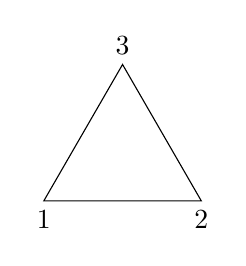
\begin{tikzpicture}
        % Dibujar el triángulo equilátero centrado en el origen
        \draw (-1,0) -- (1,0) -- (0,1.732) -- cycle;
        
        % Etiquetar los vértices
        \node[below] at (-1,0) {1};
        \node[below] at (1,0) {2};
        \node[above] at (0,1.732) {3};
    \end{tikzpicture}
\end{center}
    \begin{enumerate}
        \item Dado un triángulo rectángulo con centro en el origen de vértices $\{1,2,3\}$, isometrías que dejan fija la figura son:
            \begin{itemize}
                \item Identidad, $id$.
                \item Rotación que lleva 1 en 2 y 2 en 3 (girar $\frac{2\pi}{3}$):
                    \begin{equation*}
                        r_1 = (1\ 2\ 3)
                    \end{equation*}
                \item Rotación que lleva 3 en 2 y 2 en 1 (girar $\frac{4\pi}{3}$):
                    \begin{equation*}
                        r_2 = (1\ 3\ 2)
                    \end{equation*}
            \end{itemize}
            Simetrías axiales son por cada una de las rectas de las mediatrices de los lados:
            \begin{align*}
                s_1 &= (1\ 2) \\
                s_2 &= (1\ 3) = sr \\
                s_3 &= (2\ 3) = sr^2
            \end{align*}
        \item Pensando en el cuadrado:
            \begin{itemize}
                \item Rotaciones:
                    \begin{itemize}
                        \item Identidad.
                        \item $\frac{\pi}{2}$: $(1\ 2\ 3\ 4)=r$.
                        \item $\pi$: $(1\ 3)\ (2\ 4)=r^2$ (1 y 3 se intercambian y luego los otros).
                        \item $\frac{3\pi}{2}$: $(1\ 4\ 3\ 2)=r^3$.
                        \item $r^4 = 1$ (la identidad).
                    \end{itemize}
                \item Simetrías:
                    \begin{itemize}
                        \item Las mediatrices (2):
                            \begin{equation*}
                                s = s_1 = (1\ 2)\ (3\ 4) \qquad s_2 = (1\ 4)\ (2\ 3)
                            \end{equation*}
                        \item Unir dos vértices opuestos (2).
                            \begin{equation*}
                                s_3 =(2\ 4) \qquad s_4 = (1\ 3)
                            \end{equation*}
                            Se cumple que $s_i^2 = 1$.
                    \end{itemize}
                    Se verifica que $sr\neq rs$, pero sí se cumple $sr = r^{3}s$.
                    \begin{gather*}
                        (1\ 4)\ (2\ 3) = r^2s \\
                        (1\ 3) = r^3 s \\
                        (2\ 4) = rs
                    \end{gather*}
            \end{itemize}
    \end{enumerate}
    Si ahora pensamos en la tabla de $D_4$ (Hacer mirando la prop 1.7):
    \begin{equation*}
        \left(\begin{array}{c|cccccccc}
             & 1 & r & r^2 & r^3 & s & sr & sr^2 & sr^3 \\
             \hline
                1 & 1 & r & r^2 & r^3 & s & sr & sr^2 & sr^3 \\
                r & r & r^2 & r^3 & 1 & sr^3 & s & sr & sr^2 \\
                r^2 & r^2 & r^3 & 1 & r & sr^2 & sr^3 & s & sr \\
                r^3 & r^3 & 1 & r & r^2 & sr & sr^2 & sr^3 & s \\
                s & s & sr & sr^2 & sr^3 & 1 & r & r^2 & r^3 \\
                sr & sr & sr^2 & sr^3 & s & r^3 & 1 & r & r^2 \\
                sr^2 & sr^2 & sr^3 & s & sr & r^2 & r^3 & 1 & r \\
                sr^3 & sr^3 & s & sr & sr^2 & r & r^2 & r^3 & 1 
        \end{array}\right)
    \end{equation*}
\end{ejemplo}

Para $D_n$ en forma general:
\begin{definicion}[Grupos diédricos $D_n$]
    Consideramos $D_n$, las isometrías que dejan fijo un polígono regular de $n$ lados. Tendremos, por tanto, $2n$ elementos:
    \begin{itemize}
        \item $n$ rotaciones de ángulo $\frac{2k\pi}{n}$ con $k\in \{0,\ldots,n-1\}$.
        \item $n$ simetrías axiales:
            \begin{itemize}
                \item Si $n$ es par tenemos:
                    \begin{itemize}
                        \item $\nicefrac{n}{2}$ respecto a las mediatrices.
                        \item $\nicefrac{n}{2}$ respecto a unir vértices contrarios.
                    \end{itemize}
                \item Si $n$ es impar, tenemos $n$ respecto a las mediatrices.
            \end{itemize}
    \end{itemize}
\end{definicion}

\begin{notacion}
    Dado $D_n$, notaremos por:
    \begin{itemize}
        \item $r$ a la rotación de ángulo $\frac{2\pi}{n}$.
        \item $s$ a la simetría que pasa por el origen de coordenadas y el vértice nombrado 1.
    \end{itemize}
\end{notacion}

\begin{prop}
    Dado $n\in \mathbb{N}$, en $D_n$ se cumple que:
    \begin{enumerate}
        \item $1,r,r^2,\ldots,r^{n-1}$ son todos distintos y $r^n =1$, es decir, $O(r)=n$.
        \item $s^2 = 1$.
        \item $s\neq r^i$ $\forall 0 \leq i \leq n-1$ (ya que $s$ fija el 1).
        \item $sr^i$ con $0\leq i\leq n-1$ son simetrías en los ejes de simetrías ($s_1,s_2,\ldots,s_n$), con $sr^i \neq sr^j$.
        \item $sr = r^{-1}s$.
        \item $sr^i = r^{-i}s$.
    \end{enumerate}
\end{prop}

\begin{ejemplo}
    En $D_{12}$: $sr^9sr^6 = r^9$
\end{ejemplo}

\begin{definicion}[Conjunto de generadores de un grupo]
    Un conjunto de generadores de un grupo $G$ es un subconjunto $S\subseteq G$ tal que todo elemento $x\in G$ puede escribirse como producto finito de elementos de $S$ y de sus inversos, notaremos:
    \begin{equation*}
        G = \langle S \rangle 
    \end{equation*}
    Si $S = \{x_1,\ldots,x_n\}$, escribiremos:
    \begin{equation*}
        G = \langle x_1,\ldots,x_n \rangle 
    \end{equation*}
    En cuyo caso, diremos que $G$ está generado por $S$ y podremos expresar:
    \begin{equation*}
        x = s_1^{\gamma_1}\ldots s_p^{\gamma_p} \qquad s_i \in S, \quad \gamma_i = \pm 1
    \end{equation*}
\end{definicion}

\begin{ejemplo}
    Veamos:
    \begin{enumerate}
        \item $G=\langle x \rangle $, en cuyo caso diremos que $G$ es un grupo cíclico.
            Por ejemplo, $\mathbb{Z} = \langle 1 \rangle $ (con notación aditiva).
        \item $D_n = \langle r,s \rangle $
    \end{enumerate}
\end{ejemplo}

\begin{prop}
    Si $G=\langle S \rangle $ y existe un conjunto de relaciones $R_1,R_2,\ldots,R_m$ (igualdades entre elementos de $S\cup\{1\}$) tal que cualquier relación entre los elementos de $S$ puede deducirse de estas, entonces, decimos que estos generadores y relaciones constituyen una presentación de $G$, notado:
    \begin{equation*}
        G=\langle S / R_1,R_2,\ldots, R_n \rangle 
    \end{equation*}
\end{prop}

\begin{ejemplo}
    \begin{itemize}
        Veamos que:
        \item En el diédrico $D_n$, tenemos que:
        \begin{equation*}
            D_n = \langle r,s / rs=sr^{-1}, r^n = 1, s^2 = 1 \rangle 
        \end{equation*}
        \item $D_1 = \langle s, s^2 = 1 \rangle$.
        \item $D_2 = \langle r,s/r^2 = s^2 = 1, sr=rs \rangle$.
        \item $C_n = \langle x / x^n = 1 \rangle $ es un grupo cíclico de orden $n$.
        \item $V^{\text{abs}} = \langle x,y / x^2=1,y^2 = 1, {(xy)}^{2}=1 \rangle $ es el grupo de Klein abstracto.
        \item $Q_2^{\text{abs}} = \langle x,y/x^4 = 1, y^2 = x^2, yxy^{-1} = x \rangle $.
        \item Pensar cómo se relaciona $Q_2^{\text{abs}}$ con los cuaternios:
            \begin{equation*}
                Q_2 = \{\pm 1, \pm i, \pm j, \pm k\}
            \end{equation*}
            $i\rightarrow j\rightarrow k$ en signo positivo.
    \end{itemize}
\end{ejemplo}
